\chapter{Estudo dos Dados}
\label{cap:estudodados}


\section{Preparo dos Dados}


Para treinar algum tipo de modelo preditivo com os dados, é necessário parear
dados de entrada e de saída. Devido a dificuldades logísticas de se casar um
mesmo lote de cimento em diferentes partes do processo (e.g. no forno e na
expedição), num primeiro momento estudos serão feitos apenas para os dados de
\textit{expedição de cimento}. Embora todos os conjuntos de dados tenham sido
tratados e estudados, para algumas estatísticas serão reproduzidos aqui tabelas computadas dos
dados de expedição. O restante das estatísticas podem ser encontradas no Apêndice~\ref{ape:tables}

Segue uma breve definição de cada coluna dos dados de Expedição de Cimento: \\

\begin{itemize}
\item (i) Porcentagens relacionadas a Composição Química composition: AL\textsubscript{2}O\textsubscript{3}, SIO\textsubscript{2}, MGO, RICARB, P\textsubscript{2}O\textsubscript{5} and FE\textsubscript{2}O\textsubscript{3}
\item (ii) Porcentagem de massa de água em relação ao cimento: AGP
\item (iii) Tempo (em segundos) que o material demora para começar e terminar a endurecer, respectivamente: IP, FP
\item (iv) Blaine fineness, medido em centimetros quadrados por grama ($Cm^{2}/g)$: SBL
\item (v) Porcentagem de massa perdida no forno: FP
\item (vi) As medidas de CSC respectivamente 3, 7 e 28 dias após a expedição do lote de cimento: RC3, RC7, RC28
\end{itemize}

\subsection{Contagem de dias válidos}

Os dados da Intercement, por questões logísticas, são anotados em frequencias
diferentes. Os dados de Clínquer e Farinha são anotados por hora, já os de
Expedição de Cimento são anotados por dia (esses representando uma média de
diversos lotes experimentados).

\begin{enumerate}
    \item Os dados de  Clínquer possuem 3528 linhas de dados de 2936 dias distintos
\item Os dados de  Expedição de Cimento possuem 3650 linhas de dados de 2520 dias distintos
\item Os dados de  Farinha possuem 3530 linhas de dados de 2937 dias distintos
\item Os dados de  Cru possuem 3558 linhas de dados de 3558 dias distintos
\end{enumerate}

\subsection{Dados faltantes}
Embora tenhamos uma quantidade razoável de dias com dados presentes, esses muitas vezes não possuem algum valor de alguma coluna.
A seguir vemos para os dados de Expedição de Cimento, para cada uma de suas colunas, a porcentagem de dados presentes. 


\begin{figure}[H]
  \centering
  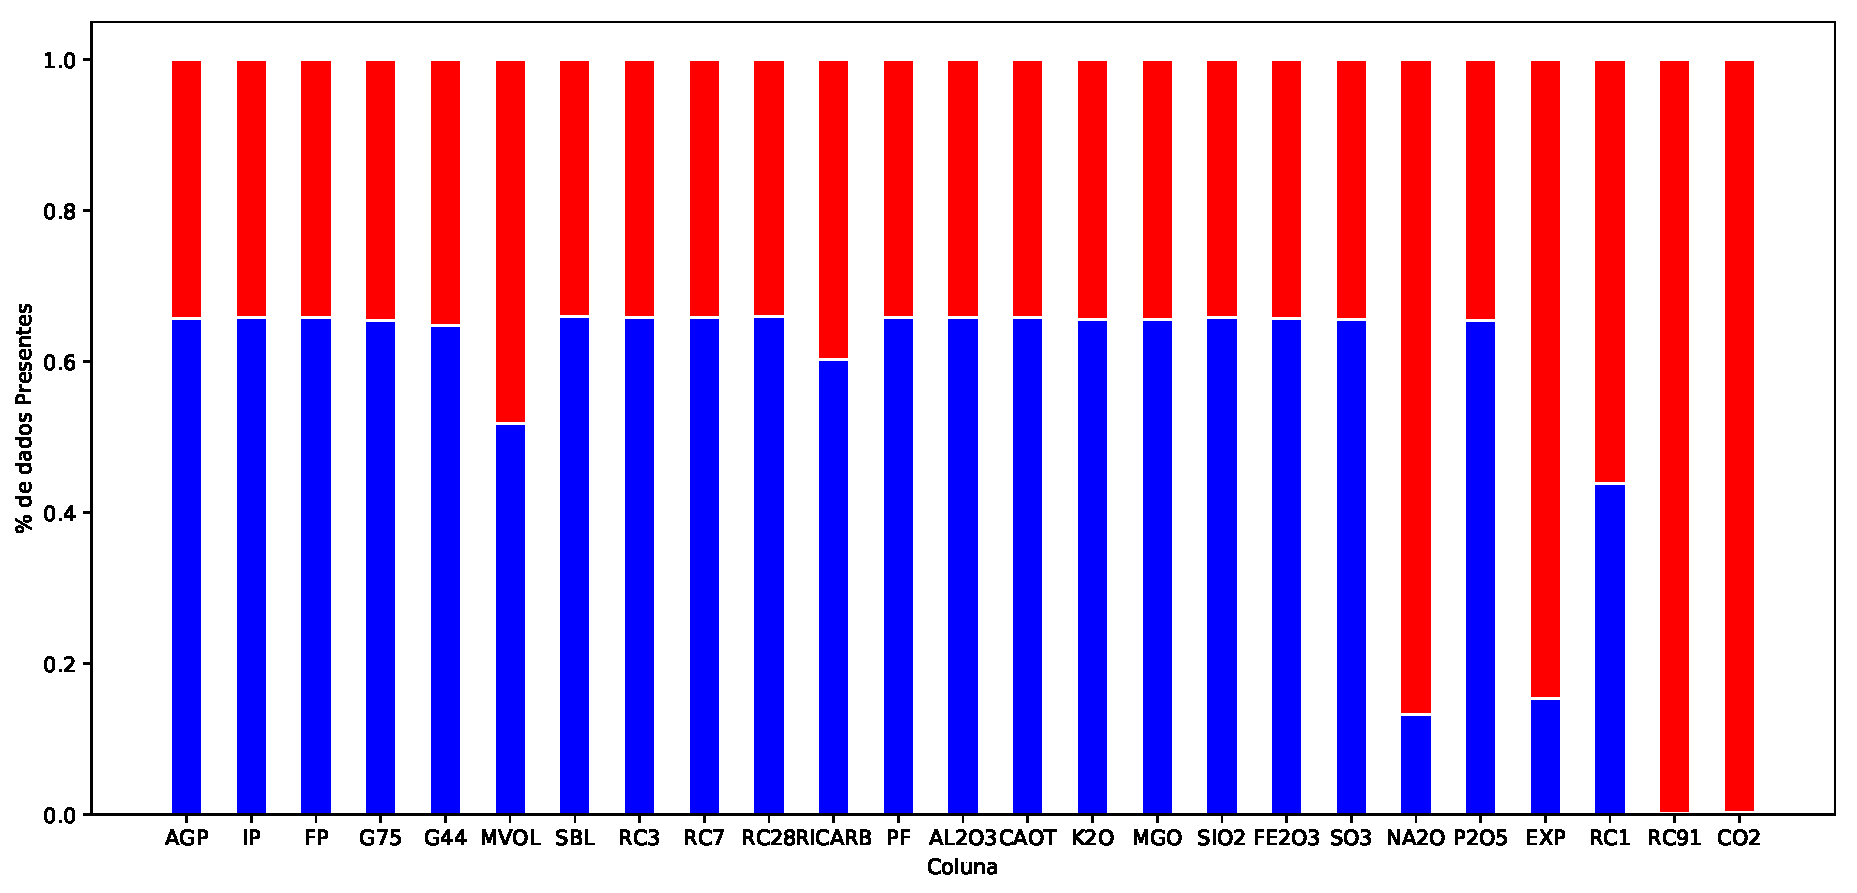
\includegraphics[width=0.9\columnwidth]{slides_dados_pct.pdf}
  \caption{Porcentagem de dados faltantes por Coluna para dados de Expedição de Cimento}
  \label{fig:dadosfalta}
\end{figure}


\section{Reamostragem dos dados}
Para maior facilidade de manuseio dos dados foi necessário realizar uma
\textbf{reamostragem}. Os dados foram modificados para que entradas realizadas no
mesmo dia sejam unidas tirando por exemplo a sua média. Além disso, dias sem
dados foram criados como placeholders para facilidade de visualização dos dados.
A seguir são reproduzidas as contagens de dados após a reamostragem.
A Figura \ref{fig:reamos} mostra como os dados estavam antes da reamostragem: 

\begin{figure}[H]
  \centering
  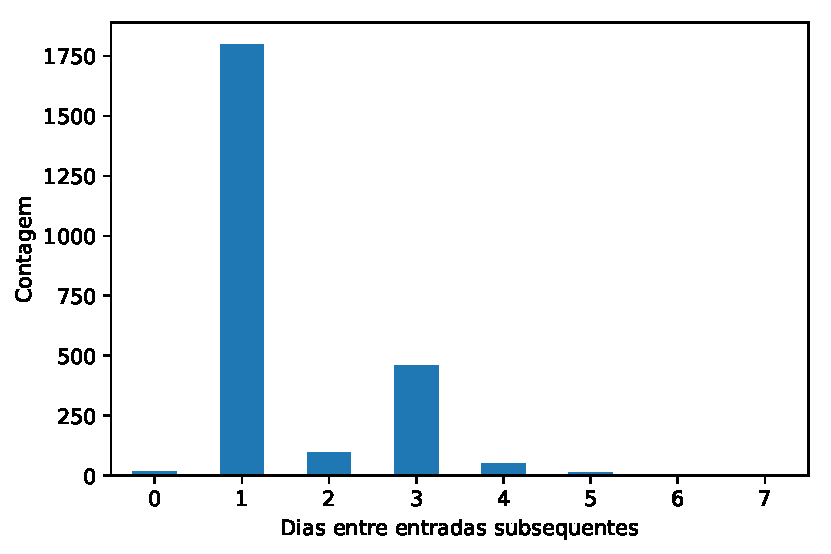
\includegraphics[width=0.5\columnwidth]{slides_dados_antes_resample.pdf}
  \caption{Distribuição das distâncias entre entradas subsequentes dos dados de Expedição de Cimento, antes da reamostragem.}
  \label{fig:reamos}
\end{figure}

\begin{itemize}
\item Clínquer: Temos dados de entrada do dia 22/04/2008 até o dia 18/12/2017
\item Clínquer: De um período de 3528 dias temos 2932 dias preenchidos com dados de entrada
\item Expedição: Temos dados de entrada do dia 02/01/2008 até o dia 29/12/2017
\item Expedição: De um período de 3650 dias temos 2520 dias preenchidos com dados de entrada
\item Farinha: Temos dados de entrada do dia 20/04/2008 até o dia 18/12/2017
\item Farinha: De um período de 3530 dias temos 2937 dias preenchidos com dados de entrada
\item Cru: Temos dados de entrada do dia 21/04/2008 até o dia 09/12/2016
\item Cru: De um período de 3155 dias temos 2675 dias preenchidos com dados de entrada
\end{itemize}


\section{Testes de Sazonalidade}

Diversas publicações recentes estudam a eficácia de modelos de Deep Learning
para predição de séries temporais, como consumo de energia elétrica
\citep{lstmbr}. Os dados estudados nesse documento são séries temporais dado que
são indexados pelo tempo, porém, resta analisar características temporais desses
dados. Como exemplo, \cite{lstmbr} usaram a informação do mês atual como
parâmetro para prever o consumo de energia elétrica. Dados que não possuem nenhuma característica temporal (i.e. a ordem não importa) seriam por exemplo provenientes de um estudo do salário recebido por uma amostra da população dados fatores como gênero, escolaridade e idade. No primeiro exemplo temos um caso de \textbf{sazonalidade} nos dados, algo que pode ser analisado em séries temporais com testes de análise espectral e auto-correlação. Para os dados desse problema, iremos testar a sazonalidade dos preditores de dureza do cimento.

\subsection{Análise Espectral}

Uma maneira de testar sazonalidade de dados indexados temporalmente é usar a
técnica de Transformada de Fourier \citep{spec}, onde podemos estudar quais
frequências dentro de um espectro podem ser usadas para decompor um sinal (i.e.
nossos dados). Para essa análise usamos os índices de dureza contidos nos dados
de expedição, de 2008 até 2014 e descartamos a parte imaginária da análise já
que nossos dados não possuem parte complexa \citep{spec}. Seguem os resultados:

\begin{figure}[H]
\centering
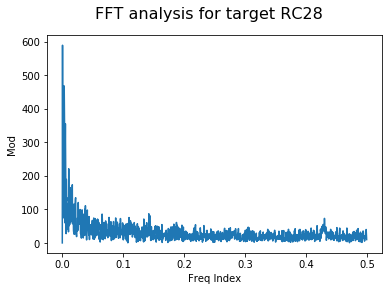
\includegraphics[width=0.9\columnwidth]{FFT_RC28.png}
\caption{Análise Espectral para preditor RC28}
\end{figure}


Podemos notar que a "energia" do sinal não possui picos em nenhuma frequência além da frequência zero, que seria a potência média do sinal, ou seja, uma componente que não depende do tempo. Então, afirmamos que esses dados não possuem sazonalidade mensal ou anual. O que significa que a média e a variância desses indicadores não possuem tendências e.g. alguma mudança similar todo mês de Janeiro.


\section{Correlação entre Colunas}

Vamos analisar agora a \textit{correlação} entre colunas dos dados de expedição
de cimento. Usaremos sempre a \textit{correlação de Pearson} para os cálculos.
\\
Sejam dois vetores de
dados $\{x_1,x_2, \dots , x_n\}$ e $\{y_1,y_2, \dots , y_n\}$, ambos com $n$ entradas. A correlação de Pearson $r$ é calculada
por meio da seguinte fórmula, onde $\overline{x}$ denota a média amostral do
vetor $X$: \\



\[ r = \frac{{}\sum_{i=1}^{n} (x_i - \overline{x})(y_i - \overline{y})}
{\sqrt{\sum_{i=1}^{n} (x_i - \overline{x})^2(y_i - \overline{y})^2}} \] 


\bigskip


A Tabela~\ref{corr3728} mostra correlação entre os índices de resistência dos dados de
expedição de cimento. \\

\begin{table}[H]
\centering
\begin{tabular}{l|lll}
\cline{2-4}
\textbf{}                  & \multicolumn{1}{l|}{RC3} & \multicolumn{1}{l|}{RC7} & \multicolumn{1}{l|}{RC28} \\ \hline
\multicolumn{1}{|l|}{RC3}  & 1                        & 0.734201                 & 0.388973                  \\ \cline{1-1}
\multicolumn{1}{|l|}{RC7}  & 0.734201                 & 1                        & 0.484725                  \\ \cline{1-1}
\multicolumn{1}{|l|}{RC28} & 0.388973                 & 0.484725                 & 1                         \\ \cline{1-1}
\end{tabular}
\caption{Correlação entre Índices de Resistência dos dados de
  Expedição de Cimento}
\label{corr3728}
\end{table}






%%% Local Variables:
%%% mode: latex
%%% TeX-master: "../quali"
%%% End:
